\Section{GAME}
\label{sec:game}

The Pokémon\textsuperscript{\textregistered} game, released for the Nintendo\textsuperscript{\textregistered} Game Boy\textsuperscript{\textregistered} in 1996 in two complementary versions, is a role-playing game based on the premise of a young man who takes the goal of finding and capturing each one of the 150 Pokémons (\textit{pocket monsters}).

The various Pokémons were attainable in different ways (some only existed in one of the versions and had to be traded), the most common being the ``tall grass'' -- one of the many visual elements to represent an area where a Pokémon could appear. Other Pokémons could only be obtained by evolving a previous form to a certain level.

The act of catching a wild Pokémon consisted in weakening it through battle (although this was often unnecessary) and using an item called PokéBall. If the Pokémon settled inside the ball, it would be considered caught. If it broke free, the battle would continue, giving the player a chance to retry. Some Pokémon were also able to flee from a battle.

The implemented game follows the same premiss but uses a mechanic different than that of the original game, thus including an interactive component with augmented reality. In this game, the markers represent the places where Pokémons can appear (``tall grass''). While a marker is visible, it is possible for a Pokémon to appear in it. If such happens, the player may hide the marker (equivalent to throwing a PokéBall). Due to the already described process of aging the markers, it takes a few frames for the action of the player to be recognized, after which the image of the Pokémon in the hidden marker changes into that of a PokéBall. Each Pokémon holds a different catch rate, and depending on the value generated in each frame, the Pokémon may settle (consequently being accepted as caught), may break free or may just shake the PokéBall. If the Pokémon is caught, the PokéBall simply disappears, and the process starts over. If the Pokémon breaks free, the player must reveal the marker and conceal it again. If the PokéBall shakes, the decision process is repeated in the next frame. A Pokémon is allowed to flee after some frames while idle or after breaking free.

\begin{figure}
	\begin{center}
		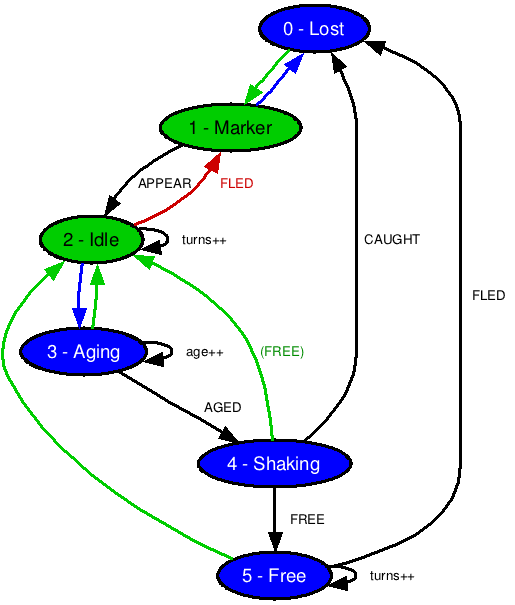
\includegraphics[width=\columnwidth]{report/images/marker.png}
	\end{center}
	\caption[Marker States]{Finite State Machine which describes the markers during the game. States in blue represent an invisible marker, states in green represent a visible one. Green and blue arrows represent a change in the marker visibility. Black and red arrows represent conditional events.}
	\label{fig:fnm}
\end{figure}

Each marker is represented in the game as a Finite State Machine, described in \Cref{fig:fnm}. The implemented states are as follows:
\begin{description}
	\item[Lost (hidden)]{Every marker starts in this state and changes only when revealed.}
	\item[Marker (revealed)]{Empty marker. If hidden, the state changes back to Lost. In each frame, a Pokémon is selected and $\xi\in\left[0,1\right]$ is generated. If $\xi$ is less than the probability for that Pokémon to appear, the Pokémon is assigned to the marker and the state changes to Idle. Otherwise it remains in the same state.}
	\item[Idle (revealed)]{The Pokémon is kept on the marker, waiting for player interaction. If the marker is hidden, the state changes to Aging. After some frames (turns) without interaction, in each frame $\xi\in\left[0,1\right]$ is generated and if $\xi$ is less than the probability for the Pokémon to flee, the Pokémon is removed from the marker and the state changes back to Marker. Otherwise it remains in the same state.}
	\item[Aging (hidden)]{As described, this state sole purpose is to compensate the lack of stability in the marker detection mechanism. Each frame the age of the marker is incremented. When the age reaches the configured threshold, the state changes to Shaking. If the marker is revealed, the state changes back to Idle.}
	\item[Shaking (hidden)]{In each frame, $\xi\in\left[0,1\right]$ is generated. If below the catch rate $c$ of the Pokémon, it is considered caught and the marker information is deleted (thus changing the state to Lost). If above $1-c$, the state is changed to Free. Otherwise, the process is repeated in the next iteration. If the marker is revealed, the Pokémon breaks free and the state is changed back to Idle.}
	\item[Free (hidden)]{If the marker is revealed, the state changes to Idle. After some frames without interaction, $\xi\in\left[0,1\right]$ is generated and if $\xi$ is below the probability of the Pokémon fleeing, the marker is deleted (thus changing the state to Lost).}
\end{description}

\begin{figure}
	\begin{center}
		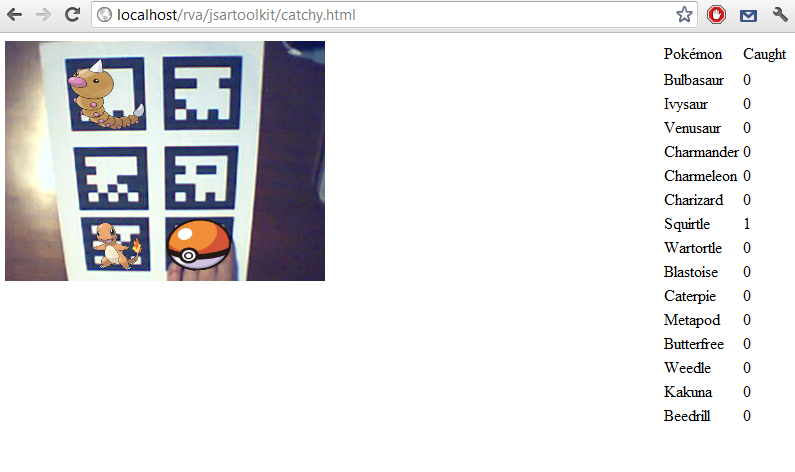
\includegraphics[width=\columnwidth]{report/images/catchy.png}
	\end{center}
	\caption[Game]{The canvas can be seen which includes the camera video feed, as well as some Pokémons appearing on randomly chosen markers. The bottom right marker is currently being obstructed by the user's hand, so a pokéball is shown instead, meaning the player is currently capturing that pokémon.}
	\label{fig:catchy}
\end{figure}

\SubSection{EVOLUTION}
\label{sec:evolution}

In order to simulate the process of evolution, the concept of level is simplified to that of how many times a form as been caught. The subsequent forms are then locked with the required number of times the previous form needs to be caught in order to unlock it. The act of unlocking is automatic: when a Pokémon is selected in the Marker state, if the number of times the previous form has been caught is greater than the lock value, the Pokémon is accepted.

As an example, assume three forms $X$, $Y$ and $Z$ where $Y$ is the evolution of $X$ and $Z$ is the evolution of $Y$. Also, assume $C_{F}$ and $L_{F}$ to be the number of times the form $F$ has been caught and the lock value of the form $F$, respectively. Since $X$ is the base form, $L_{X}=0$. If $L_{Y}=y$, it means that the form $Y$ will not appear while $C_{X}<y$. Similarly, if $L_{Z}=z$, the form $Z$ will not appear while $C_{Y}<z$.
\SubSection{POKÉDEX}
\label{sec:pokedex}

In the original game, the player is able to keep track of the Pokémons he/she has caught using the Pokédex, a fictional device which records the informations about all the seen and caught Pokémons in a numbered list.

Since a similar logic feature was required to implement the evolution system, a \texttt{table} tag was added to the page of the game with the scoreboard of each Pokémon. This table is automatically updated using the Document Object Model\footnote{(DOM) Convention used to access the elements of an HTML page using an object-oriented paradigm, regarding the scripting language used.} methods.
